\documentclass[runningheads]{llncs}
\usepackage[T1]{fontenc}
\usepackage{lmodern}
\usepackage{amsmath,amssymb}
\usepackage{graphicx}
\usepackage[labelformat=parens,labelsep=space,font=footnotesize]{subcaption}
\usepackage{booktabs}
\usepackage{xcolor}
\usepackage{xurl}
\usepackage[hidelinks]{hyperref}

% \TBD{...} marks a value that must be filled before submission. With
% \pendingfalse any remaining \TBD stops the build.
\emergencystretch=1.5em
\newif\ifpending \pendingtrue
\newcommand{\TBD}[1]{\ifpending\textcolor{red}{\textbf{[TBD: #1]}}\else\errmessage{Unfilled TBD: #1}\fi}

\begin{document}

\title{Early Warning for Cross-Chain DeFi Laundering: Scoring Trajectory Prefixes with Typed Temporal Motifs}
\titlerunning{Early Warning for Cross-Chain DeFi Laundering}
\author{Anonymous Author(s)}
\authorrunning{Anonymous}
\institute{Anonymous Institution}

\maketitle

\begin{abstract}
After a DeFi exploit, stolen funds are laundered through fresh wallets, DEX swaps, splits and bridge or mixer deposits, often within minutes.
Cross-chain tracers reconstruct such flows after the fact; they do not tell an analyst, while the flow unfolds, whether it is heading for an exit that cannot be undone.
We present CAGI-ED, a CPU-only pipeline that monitors a seed address, decodes every new action into a DeFi semantic type, expands the tainted value flow, and re-scores the growing trajectory prefix with a calibrated gradient-boosted model whose alerts carry TreeSHAP evidence mapped to MITRE AADAPT techniques.
We rebuilt a dataset of 15 publicly documented cross-chain incidents on Ethereum, BNB Smart Chain and Arbitrum with 393 hard negatives mined from the same bridges, DEXs and mixers, and evaluate with leave-one-incident-out and incident-level bootstrap.
Replaying each trajectory action by action, the calibrated detector alerts on 12 of 15 incidents while 5.8\% of multi-action hard negatives raise a false alert; where the exit is not the very first action, it warns before the exit in three of six incidents, 5 to 114 minutes early.
One minute after the first action, typed features double PR-AUC over the same learner on type-agnostic features (0.42 vs.\ 0.22, paired $p=0.01$); over all prefixes the two are statistically indistinguishable (0.48 vs.\ 0.52), and both far exceed a rule-based typology score (0.21).
Platt scaling reduces the expected calibration error from 0.071 to 0.015, and scoring a prefix takes 12 to 24\,ms.
We release the raw evidence cache, the decoded trajectories and one-command scripts for every number.
\keywords{Cross-chain laundering \and Early detection \and DeFi security \and Temporal motifs \and Blockchain forensics}
\end{abstract}

%=============================================================================
\section{Introduction}
\label{sec:intro}
%=============================================================================

Cross-chain bridges move assets between heterogeneous ledgers and have become core infrastructure of decentralized finance (DeFi)~\cite{robinson2021survey,ou2022overview}.
They are also a preferred laundering route.
Bridge exploits account for many of the largest thefts in the ecosystem~\cite{lee2023sok}, and Elliptic estimates that more than \$21 billion of criminal and high-risk funds had passed through DEXs, bridges and swap services by 2025, a threefold rise over two years~\cite{elliptic2025crosschain}.
After an exploit, the attacker typically moves the proceeds within hours: fresh intermediary wallets, token swaps into liquid assets, fan-out splits, and finally a bridge deposit, a mixer or an exchange, after which the trail is lost or frozen funds can no longer be recovered.
MITRE's AADAPT framework names these steps cross-chain hopping, layering, peel chains and anonymizing services~\cite{mitre2025aadapt}.

Research has made steady progress on \emph{reconstructing} such flows.
CONNECTOR and ABCTracer associate deposits and withdrawals across bridges~\cite{lin2025connector,lin2025abctracer}, BridgeGuard and XChainWatcher detect attack transactions and rule violations on bridges~\cite{wu2025safeguarding,augusto2025xchainwatcher}, and AMLGuard combines semantic transaction analysis with retrieval-augmented language-model reasoning to trace laundering paths on 82 real cases~\cite{wu2026amlguard}.
These systems answer a forensic question, \emph{where did the money go?}, and they work on complete or nearly complete histories.
A compliance team, a bridge operator or an exchange facing an incident \emph{while it unfolds} needs a different answer: given only the actions observed so far, is this flow on a laundering path, and how much time is left before it reaches an exit that cannot be undone?

We call this problem \emph{early detection of cross-chain laundering} and study it on real incidents.
It differs from forensic tracing in three ways.
First, the detector sees only a prefix of the trajectory and must score it without any information that depends on how the trajectory ends.
Second, most prefixes of benign activity look like laundering: a user who bridges, swaps and splits is not a thief, so the detector must be evaluated against benign trajectories that pass through the same bridges at the same time.
Third, a score is only useful if it is calibrated and explained, because a human decides whether to freeze or escalate.

We present \textbf{CAGI-ED} (Cross-chain Attack Graph Intelligence for Early Detection), a CPU-only pipeline that monitors a seed address, decodes every new action into a DeFi semantic type (transfer, swap, bridge, lending, split, merge, mixer or exit), expands the tainted value flow, and re-scores the growing trajectory after each action.
The scorer uses \emph{typed temporal motifs}, features that describe what kind of actions happened, in which order and how fast, and turns them into a calibrated probability with an explanation in AADAPT terms.

\paragraph{Contributions.}
\begin{itemize}
\item \textbf{Problem and protocol.} We formalize prefix-based early detection with an explicit endpoint, lead time and per-trajectory false-alert rate, and we separate online horizons (available to a live monitor) from relative checkpoints (a retrospective diagnostic). We evaluate under leave-one-incident-out with incident-level bootstrap intervals, and we report a leak that we found and removed in our own earlier pipeline (Sect.~\ref{sec:problem},~\ref{sec:setup}).
\item \textbf{System.} An end-to-end architecture from multi-chain explorer APIs to explained alerts: an evidence cache with checksums, a semantic decoder over a verified protocol map, a bounded value-flow trajectory builder, 37 prefix-safe features in three groups, and a calibrated gradient-boosted scorer with TreeSHAP attributions mapped to MITRE AADAPT (Sect.~\ref{sec:method}).
\item \textbf{Dataset.} 15 publicly documented cross-chain incidents (2021--2025) on Ethereum, BNB Smart Chain and Arbitrum, each traced from its seed, with 393 hard-negative trajectories mined from the same bridges, DEXs and mixers in the same time window. We release the decoded trajectories, the raw evidence cache and all scripts (Sect.~\ref{sec:data}).
\item \textbf{Evidence.} A controlled study that holds the learner fixed and varies only the representation, results at online horizons from one minute to one day, lead time and false alerts per threshold, ablations, calibration, a mimicry stress test and cost on commodity hardware (Sect.~\ref{sec:results}).
\end{itemize}
%=============================================================================
\section{Related Work}
\label{sec:related}
%=============================================================================

\paragraph{Cross-chain tracing and bridge security.}
Surveys describe the diversity of cross-chain protocols~\cite{robinson2021survey,ou2022overview}, and Lee et al.\ systematize bridge hacks and their losses~\cite{lee2023sok}.
Xscope checks cross-chain invariants to find bridge attacks~\cite{zhang2022xscope}, SmartAxe finds vulnerabilities in bridge contracts by static analysis~\cite{liao2024smartaxe}, XChainWatcher monitors bridges with Datalog rules~\cite{augusto2025xchainwatcher}, and BridgeGuard characterizes and detects attack transactions~\cite{wu2025safeguarding}.
These systems protect the bridge itself; CAGI-ED starts after the exploit and follows the stolen value.
For tracing, Yan et al.\ match Ethereum--Polygon transfers~\cite{yan2025tracing}, CONNECTOR automates deposit--withdrawal association~\cite{lin2025connector}, and ABCTracer generalizes it to bidirectional tracing across 12 bridges~\cite{lin2025abctracer}.
Their output, a matched pair of transactions, is an input that CAGI-ED could consume to continue a trajectory on the destination chain.
Such links are not always recoverable: privacy-preserving cross-chain swap protocols such as zk-HTLC are designed to defeat linkability attacks between the two legs of an exchange~\cite{tran2026zkhtlc}.
This is one reason CAGI-ED treats the bridge deposit on the source chain as the endpoint and aims to alert before it.

\paragraph{Laundering detection on account-based chains.}
DenseFlow finds laundering accounts in Ethereum by locating dense value flows~\cite{lin2024denseflow}, and address-clustering heuristics link accounts controlled by the same entity~\cite{victor2020clustering}.
AMLGuard is closest to our work: it parses transactions into DeFi semantic units and uses retrieval-augmented reasoning to reconstruct a compact illicit-flow topology across chains~\cite{wu2026amlguard}.
CAGI-ED differs in its task and its output.
It scores \emph{partial} trajectories and outputs a \emph{calibrated} probability, an alert time and its evidence, not a topology; it runs on a CPU without a language model; and it is evaluated against hard negatives that use the same protocols.
The two are complementary: AMLGuard-style reconstruction can supply seeds and labels, and CAGI-ED can monitor new incidents before reconstruction is possible.

\paragraph{Graph learning for illicit activity.}
Graph convolutional networks on the Elliptic dataset~\cite{weber2019elliptic}, Elliptic++~\cite{elmougy2023ellipticpp} and the subgraph-level Elliptic2~\cite{bellei2024elliptic2} established graph learning for Bitcoin anti-money laundering.
Multi-relational~\cite{hyun2023aml}, temporal~\cite{alarab2023graphlstm,patel2022evangcn} and sequence-pretrained~\cite{li2022ttagn,hu2023bert4eth} models extend it to Ethereum phishing and fraud, and temporal graph networks give a general dynamic-graph backbone~\cite{rossi2020tgn}.
These methods need thousands of labeled nodes or subgraphs on one ledger and score complete histories.
With 15 incidents we deliberately use a small, interpretable tree ensemble and report where the evidence is and is not conclusive.

\paragraph{Early classification.}
Early classification of time series trades accuracy for earliness by deciding on a prefix~\cite{xing2012early,gupta2020early}.
We adopt its prefix view but measure earliness against a domain event, the laundering endpoint, and report false alerts per benign trajectory because every alert costs an analyst's time.

Table~\ref{tab:positioning} summarizes the closest systems.

\begin{table}[t]
\centering
\caption{Positioning against the closest systems. ``Laund.\ path'': models multi-step post-exploit flows; ``Prefix'': emits a decision before the flow completes; ``Calib.'': outputs a calibrated probability.}
\label{tab:positioning}
\setlength{\tabcolsep}{3pt}
\small
\resizebox{\linewidth}{!}{%
\begin{tabular}{@{}llp{2.9cm}ccccp{1.5cm}@{}}
\toprule
System & Year & Primary task & X-chain & Laund. path & Prefix & Calib. & Evidence \\
\midrule
DenseFlow~\cite{lin2024denseflow} & 2024 & Laundering accounts & No & Yes & No & No & Flow subgraph \\
CONNECTOR~\cite{lin2025connector} & 2025 & Bridge tx association & Yes & No & No & No & Matched pair \\
ABCTracer~\cite{lin2025abctracer} & 2025 & Bidirectional tracing & Yes & No & No & No & Matched pair \\
BridgeGuard~\cite{wu2025safeguarding} & 2025 & Bridge attack tx detection & Yes & No & No & No & -- \\
XChainWatcher~\cite{augusto2025xchainwatcher} & 2025 & Bridge anomaly rules & Yes & No & Online & No & Violated rule \\
AMLGuard~\cite{wu2026amlguard} & 2026 & LLM-aided laundering tracing & Yes & Yes & No & No & Flow topology \\
\textbf{CAGI-ED} & -- & Early laundering alert & Yes & Yes & Yes & Yes & SHAP + AADAPT \\
\bottomrule
\end{tabular}}
\end{table}
%=============================================================================
\section{Problem Formulation}
\label{sec:problem}
%=============================================================================

\paragraph{Typed events.}
Let $\mathcal{C}=\{\text{Ethereum},\text{BSC},\text{Arbitrum}\}$.
A decoded action is a tuple $a=(t,c,u,v,y,\kappa,q,\pi)$ with timestamp $t$, chain $c\in\mathcal{C}$, source and destination addresses $u,v$, semantic type $y\in\mathcal{Y}$, token $\kappa$, log-scaled amount $q=\log(1+\text{amount})$ and protocol label $\pi$ (empty for plain transfers).
The type vocabulary is
\begin{align*}
\mathcal{Y}=\{&\textsf{transfer},\textsf{swap},\textsf{bridge\_dep},\textsf{bridge\_wdr},\textsf{lend\_dep},\\
&\textsf{lend\_wdr},\textsf{split},\textsf{merge},\textsf{mixer/exit},\textsf{other}\}.
\end{align*}

\paragraph{Trajectories and prefixes.}
Starting from a seed address $s$ named in a public incident report (or, for a negative, an address matched to the incident, Sect.~\ref{sec:data}), a trajectory $\tau=(a_1,\dots,a_n)$ is the time-ordered sequence of actions reached by bounded value-flow expansion (Sect.~\ref{sec:traj}).
The prefix of length $k$ is $\tau_{1:k}=(a_1,\dots,a_k)$; at wall-clock time $t$ the monitor has observed $\tau_{1:k(t)}$ with $k(t)=|\{i: t_i\le t\}|$.

\paragraph{Endpoint and lead time.}
For an incident trajectory whose exit is confirmed by a public source, the endpoint index $e^\star$ is the first action whose type is \textsf{bridge\_dep}, \textsf{lend\_dep} or \textsf{mixer/exit}, i.e.\ the first step after which the funds leave the monitored chain or enter a pool that breaks the trace; $t_e=t_{e^\star}$.
A detector outputs $\hat p_k=\Pr(\text{laundering}\mid\tau_{1:k})$ from $a_1,\dots,a_k$ only.
Given a threshold $\theta$, the first alert is at $k_a=\min\{k\ge2:\hat p_k\ge\theta\}$ and
\begin{equation}
\text{lead time}=t_e-t_{k_a},\qquad \text{lead steps}=e^\star-k_a .
\label{eq:lead}
\end{equation}
An alert with $k_a\ge e^\star$ is \emph{late}; late alerts are counted separately and never enter lead-time statistics.
An alert on a negative trajectory at any $k$ is a false alert, so false-alert rates are per trajectory, not per prefix.

\paragraph{Two views of ``early''.}
We evaluate two families of prefixes.
\emph{Online horizons} $k(t_1+h)$ for $h\in\{1\,\text{min},\dots,24\,\text{h}\}$ are available to a live monitor.
\emph{Relative checkpoints} $k=\lceil r n\rceil$, $r\in\{25,50,75,100\}\%$, require the final length $n$ and are therefore a retrospective diagnostic only; they are never used as a model input (a feature equal to $k/n$ was removed after we found it leaked $n$, Sect.~\ref{sec:features}).

\paragraph{Threat model and scope.}
The adversary controls pseudonymous addresses holding stolen or illicit funds and may use any public bridge, DEX, lending market or mixer.
The defender knows one seed address from a public report and observes public chain data only.
Breaking mixer anonymity, discovering incidents by whole-chain scanning, and attributing real-world identities are out of scope.

%=============================================================================
\section{The CAGI-ED Architecture}
\label{sec:method}
%=============================================================================

Figure~\ref{fig:arch} shows the four layers of CAGI-ED: (i) a multi-chain collector with an evidence cache, (ii) a semantic decoder that turns raw transfers into typed actions, (iii) a trajectory builder that follows tainted value from the seed, and (iv) an online scorer that recomputes prefix features on every new action, calibrates the score and emits an explained alert.

\begin{figure}[t]
\centering
\IfFileExists{figures/fig1_architecture.pdf}{\includegraphics[width=\linewidth]{figures/fig1_architecture.pdf}}{\fbox{\parbox[c][4.2cm][c]{0.95\linewidth}{\centering Figure 1 (architecture, drawn in draw.io): see \texttt{paper/figures/fig1\_architecture.pdf}}}}
\caption{CAGI-ED architecture. Raw explorer responses are cached with checksums, decoded into typed actions using a verified protocol map, and expanded from the seed into a value-flow trajectory. On every new action the scorer recomputes the prefix feature vector $\mathbf{x}(\tau_{1:k})$, applies the gradient-boosted model $f$ and Platt calibration, and raises an alert with its top TreeSHAP contributions and AADAPT technique IDs once $\hat p_k\ge\theta$.}
\label{fig:arch}
\end{figure}

\subsection{Collection and Evidence Cache}
For Ethereum and Arbitrum the collector calls the Etherscan V2 account endpoints (normal, internal and ERC-20 transactions) with block-range pagination; for BSC it calls NodeReal's \texttt{nr\_getAssetTransfers} in both directions.
Every response is stored verbatim with its request time and SHA-256 checksum under \emph{(chain, address, incident)}, so two incidents that touch the same infrastructure never overwrite each other's evidence and every feature value can be traced back to the bytes it was computed from.
The collection window is $[b_0, b_0+72\,\text{h}]$ from the incident's start block $b_0$.

\subsection{Semantic Decoding}
A protocol map lists contracts whose role was verified on-chain (by event signature or function selector) or in explorer labels: 9 bridge endpoints of 8 families, 6 DEX routers and pools, 2 mixers and 1 lending market.
Each raw leg becomes a canonical action; legs of the same transaction are then merged into one semantic action when the structure is unambiguous: two or more tokens moving in and out of the same address form a \textsf{swap}; one source paying two or more destinations forms a \textsf{split}; two or more sources paying one destination form a \textsf{merge}.
A deposit to a verified bridge (lending market, mixer) becomes \textsf{bridge\_dep} (\textsf{lend\_dep}, \textsf{mixer/exit}) regardless of the merge rule.
Duplicate legs returned by overlapping pages are removed on (chain, transaction hash, log index).

\subsection{Bounded Value-Flow Trajectories}
\label{sec:traj}
Let $A$ be the decoded actions of the processed addresses inside the window, sorted by time, and let $\rho(a)=\mathrm{e}^{q}-1$ recover the raw amount.
For a source $u$ and token $\kappa$ write $O(u,\kappa)=\sum_{a\in A:\,u_a=u,\kappa_a=\kappa}\rho(a)$.
The builder keeps a depth map $d(\cdot)$ with $d(s)=0$ and accepts action $a$ iff
\begin{equation}
d(u_a)<D,\qquad t_a-t_1\le H,\qquad \frac{\rho(a)}{O(u_a,\kappa_a)}\ge\eta \;\;\lor\;\; \{u_a,v_a\}\cap\mathcal{P}\neq\emptyset,
\label{eq:builder}
\end{equation}
where $\mathcal{P}$ is the set of verified protocol contracts; on acceptance $d(v_a)\leftarrow\min(d(v_a),d(u_a)+1)$ unless $v_a\in\mathcal{P}$, so the expansion never walks \emph{through} shared infrastructure.
The collector then fetches the new frontier $\{v_a\}\setminus\mathcal{P}$ and the builder is re-run until the frontier is empty.
We use $D=6$ hops, $H=72$\,h and $\eta=5\%$ for incidents and $D=2$ for negatives, whose seeds are ordinary users.
The value share is computed per token so that a large stablecoin payment is not diluted by a small ETH fee.
Traces are followed on the incident's primary chain; the continuation on the destination chain of a bridge deposit is not stitched into the trajectory, because the reports we rely on confirm the exit but seldom give the destination address.
This is why a bridge deposit is a natural endpoint in our formulation.

\subsection{Prefix-Safe Features}
\label{sec:features}
For each prefix the extractor computes $\mathbf{x}(\tau_{1:k})$ from $a_1,\dots,a_k$ only (37 model inputs in total).
A unit test enforces this: two trajectories that share the first $k$ actions but differ afterwards, in content or in length, must yield identical features at $k$.
The same test caught a \emph{relative-position} feature $k/n$ in an earlier version of the code, whose denominator is the final length; it is removed, and every result in this paper is computed without it.

\begin{itemize}
\item \textbf{Flat (14).} Temporal: mean and standard deviation of inter-action gaps $\delta_i=t_{i}-t_{i-1}$, burstiness $B=(\sigma_\delta-\mu_\delta)/(\sigma_\delta+\mu_\delta)$~\cite{goh2008burstiness}, active duration $t_k-t_1$.
Structural: fan-out and fan-in of the seed, number of distinct counterparties, edge density $|E|/(|V|(|V|-1))$, maximum hop depth from the seed, number of branching addresses (out-degree $>1$).
Economic: mean of $\log(1+q_i)$, out/in value ratio, value retention $q_k/q_1$, and the number of tokens holding at least 1\% of the observed value.
\item \textbf{Typed actions (16).} The share $\frac1k|\{i\le k:y_i=y\}|$ of each type $y\in\mathcal{Y}$, the number of distinct type bigrams and trigrams, the number of distinct bridge families, the number of bridge$\to$swap transitions, the number of stablecoin legs, and the time to the first bridge action.
Raw counts are not used because they sum to $k$ and would re-introduce prefix length as a shortcut.
\item \textbf{Motifs (7).} Counted only when complete within the prefix. \emph{Split}: addresses with $\ge2$ outgoing actions; \emph{merge}: addresses with $\ge2$ incoming actions; \emph{peel chain}: a run of $\ge3$ consecutive transfers $a_{i-1}\to a_i$ with $v_{i-1}=u_i$ and $q_i\le q_{i-1}$; \emph{bridge$\to$swap} and \emph{swap$\to$split}: the ordered pair in consecutive actions; \emph{nested bridge}: $\ge2$ distinct bridge protocols; \emph{rapid token pivot}: the number of token changes between consecutive actions.
\end{itemize}
The flat group is exactly the information a type-agnostic transaction graph offers; the other two groups require the decoder.
Table~\ref{tab:aadapt} maps the observables to MITRE AADAPT~\cite{mitre2025aadapt} techniques so that an alert can be phrased in a responder's vocabulary.

\begin{table}[t]
\centering
\caption{CAGI-ED observables mapped to MITRE AADAPT techniques.}
\label{tab:aadapt}
\setlength{\tabcolsep}{4pt}
\small
\begin{tabular}{@{}llp{5.1cm}@{}}
\toprule
AADAPT ID & Technique & CAGI-ED observable \\
\midrule
ADT3005 & Cross-Chain Swaps (Hopping) & bridge deposit share, bridge$\to$swap, nested bridge \\
ADT3028 & Siphon Funds & split, fan-out, distinct counterparties \\
ADT3028.001 & Anonymous Wallets & hop depth through fresh intermediaries \\
ADT3028.003 & Layering & swap share, rapid token pivot, bigram diversity \\
ADT3028.005 & Peel Chains & peel chain, value retention \\
ADT3030 & Use Anonymizing Services & mixer/exit action (endpoint) \\
\bottomrule
\end{tabular}
\end{table}

\subsection{Scoring, Calibration and Explained Alerts}
\label{sec:scoring}
The scorer $f$ is a gradient-boosted tree ensemble (XGBoost~\cite{chen2016xgboost}, 200 trees of depth 4, learning rate 0.1, class weight $n_-/n_+$ computed on the training fold), fixed before any experiment and never tuned on the evaluation data.
Inside each training fold, features present in fewer than two positive incidents are dropped, so a feature cannot memorize one incident.
Raw scores are mapped to probabilities by Platt scaling~\cite{niculescu2005calibration},
\begin{equation}
\hat p_k=\sigma\!\bigl(\alpha\,\mathrm{logit}\,f(\mathbf{x}(\tau_{1:k}))+\beta\bigr),
\label{eq:platt}
\end{equation}
with $(\alpha,\beta)$ fitted on out-of-fold scores of the training incidents only.
When $\hat p_k\ge\theta$ for the first time, the alert carries the $k$ with the largest exact TreeSHAP contributions~\cite{lundberg2020treeshap} $\phi_j(\mathbf{x})$, where $\mathrm{logit}\,f(\mathbf{x})=\phi_0+\sum_j\phi_j(\mathbf{x})$, together with the AADAPT IDs of their features.
Because features are recomputed from the prefix, scoring is stateless and can be repeated on every block.
%=============================================================================
\section{Dataset}
\label{sec:data}
%=============================================================================

\paragraph{Incidents.}
We collected 15 cross-chain DeFi incidents from 2021 to 2025 that are documented by at least one public security source (CertiK, SlowMist, Beosin, BlockSec, PeckShield, Halborn, Chainalysis or Elliptic): 7 on BSC, 6 on Arbitrum and 2 on Ethereum (Appendix~\ref{app:incidents}).
The 82-case list of AMLGuard~\cite{wu2026amlguard} was used only to locate candidates; every seed address, start block and exit was verified on-chain by the authors against the public report.
For 12 incidents a public report confirms the exit (bridge, mixer or lending deposit); for 10 of them the exit action lies inside our trace and defines the endpoint of Sect.~\ref{sec:problem}. The other incidents are used for detection but not for lead time.

\paragraph{Hard negatives.}
A detector that separates stolen funds from dormant wallets is useless in practice, because an analyst watching a bridge sees mostly legitimate users.
We therefore mine negatives from the \emph{same} protocols and time window as each incident.
For each incident we list the verified bridge, DEX and mixer contracts on its trace and collect every counterparty of these contracts within $\pm7$ days.
A candidate is accepted if it interacted directly with the contract, received or sent a positive value, did not fan out to more than three addresses (split-like pattern), and made no mixer deposit after a non-mixer interaction.
Seeds of all incidents and the 82 AMLGuard addresses are excluded.
A second pass targets complex benign activity: it requires at least $\mathrm{e}^{0.35\log(1+n^+)}-1$ raw events, where $n^+$ is the length of the incident trajectory, and relaxes the fan-out bound on a log scale for incidents with a large fan-out.
Five manually selected controls, one per early incident (for example, a legitimate Ronin withdrawal followed by a swap in the same hour), complete the set.
Each negative is expanded with exactly the same collector, builder and depth as the incidents.

\paragraph{Collection and completeness.}
We re-collected all raw data for this paper through the free tiers of Etherscan (Ethereum, Arbitrum) and NodeReal (BSC): 43{,}080 cached responses totalling 1.5\,GB.
A trajectory enters the dataset only if every address it reaches has a complete cache.
The monthly NodeReal quota ran out before all BSC negatives were collected, so 223 of the 272 BSC negatives in the mining registry are excluded, and for one BSC incident (Paraluni) the trajectory is rebuilt from our earlier decoded trace of the same seed and window, truncated to the same depth.
No transaction appears in two incident groups; a few infrastructure addresses (routers, pools, exchange wallets) are shared, which cannot leak labels because no feature encodes address identity.

\paragraph{Statistics.}
Table~\ref{tab:data} summarizes the dataset and Fig.~\ref{fig:data} contrasts incidents with negatives.
Incident trajectories are longer (median 40 vs.\ 2 actions; 187 negatives consist of a single action) and richer in swaps and bridge deposits; because raw action counts and prefix length are not model inputs and checkpoints are evaluated separately, length alone cannot explain the results (Sect.~\ref{sec:results}).

\begin{table}[t]
\centering
\caption{Real-data statistics. Prefix rows are extracted at $k\in\{2,3,5,7\}$ and at 25/50/75/100\% of each trajectory; duplicates of the same (trajectory, $k$) are pooled once.}
\label{tab:data}
\small
\begin{tabular}{@{}lrrrr@{}}
\toprule
 & Ethereum & BSC & Arbitrum & Total \\
\midrule
Incidents & 2 & 8 & 5 & 15 \\
Hard negatives & 117 & 51 & 225 & 393 \\
Actions & 1{,}262 & 4{,}376 & 6{,}083 & 11{,}721 \\
Prefix rows (pooled, deduplicated) & & & & 1{,}384 \\
Positive rate of pooled rows & & & & 8.4\% \\
\bottomrule
\end{tabular}
\end{table}

\begin{figure}[t]
\centering
\begin{subfigure}[t]{0.49\linewidth}\centering
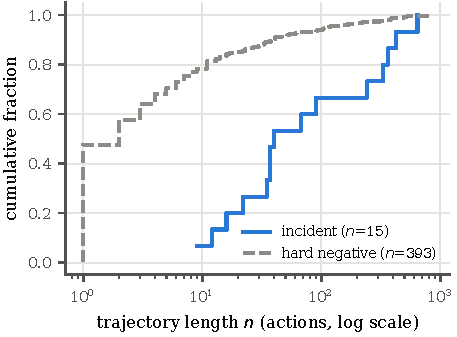
\includegraphics[width=\linewidth]{figures/fig2a.pdf}
\caption{Trajectory length (ECDF).}
\label{fig:2a}
\end{subfigure}\hfill
\begin{subfigure}[t]{0.49\linewidth}\centering
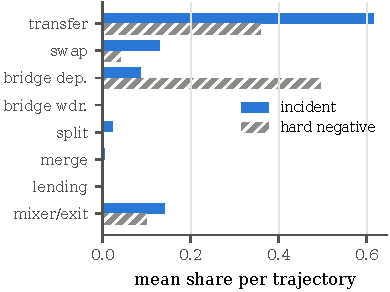
\includegraphics[width=\linewidth]{figures/fig2b.pdf}
\caption{Mean share of each action type.}
\label{fig:2b}
\end{subfigure}
\caption{Incidents versus hard negatives in the real dataset.}
\label{fig:data}
\end{figure}

\paragraph{Synthetic benchmark (CAGI-Synth).}
Fifteen incidents limit statistical power, and the real negatives cannot be made harder on demand.
We therefore also release a \emph{synthetic} benchmark, reported separately from every real-data result.
Its generator samples laundering trajectories from five typologies taken from public reports and AADAPT (peel chain to a bridge; split, swap to a stablecoin and bridge; swap and fixed-denomination mixer deposits; nested bridges; lending round trip), and benign trajectories from six ordinary behaviours (bridge user, DEX trader, payroll split, consolidation, arbitrage bot, single mixer deposit) padded with routine activity so that lengths overlap.
A difficulty knob $d\in[0,1]$ controls two things: with probability $d$ a benign trajectory is drawn from laundering-like behaviours (bridge, swap and split within minutes; hop through fresh wallets to a bridge; fast rotation of funds), and with probability $d$ per step the launderer inserts small decoy transfers and slows down.
We generate 30 synthetic incidents with 40 negatives each at $d\in\{0,0.25,0.5,0.75,1\}$.
%=============================================================================
\section{Experimental Setup}
\label{sec:setup}
%=============================================================================

\paragraph{Research questions.}
\textbf{RQ1} Does typing the actions and adding motifs improve detection over a type-agnostic view of the same flow?
\textbf{RQ2} How early can laundering be detected, measured by online horizon, lead time before the endpoint and false alerts on hard negatives?
\textbf{RQ3} Are the scores calibrated and explainable, and how robust are they to ablations, mimicry and builder settings?
\textbf{RQ4} Is the pipeline practical on commodity hardware, and is next-action forecasting supported by the data?

\paragraph{Detectors.}
\textbf{B0} predicts the training prevalence.
\textbf{B1} is a hand-weighted typology score over motif counts (bridge$\to$swap, swap$\to$split, split, nested bridge, peel chain, token pivot); it needs no training.
\textbf{B2} is logistic regression on the action-type shares (bag of actions).
\textbf{B3} is a random forest (200 trees, depth 8, balanced classes) on the 14 flat features.
\textbf{B3$'$} is \emph{the same XGBoost learner as M1}, with the same hyperparameters, class weighting, coverage filter and seed, on the 14 flat features; M1 and B3$'$ therefore differ only in the representation.
\textbf{S1} is a GRU (embedding 16, hidden 32, 25 epochs, class-weighted loss) over the last 64 typed tokens of the prefix, where a token combines the action type with a log-scale bucket of the gap to the previous action; it tests whether a sequence model learns the typed structure without hand-crafted motifs.
\textbf{M1} is CAGI-ED's scorer on all 37 features (Sect.~\ref{sec:scoring}).
The representation study adds typed-action and motif groups one at a time to the flat set with the learner fixed.
We do not re-run CONNECTOR or ABCTracer: they associate bridge transactions and output matched pairs, not laundering probabilities.

\paragraph{Protocol.}
All results use leave-one-incident-out (LOIO): in each of the 15 folds, the incident and all negatives mined for it are held out and every model, calibrator and feature filter is fitted on the other 14 groups.
Platt and isotonic calibrators are fitted on inner LOIO scores of the training groups only.
Prefix rows of the same (trajectory, $k$) that arise from several checkpoints are pooled once.
The primary metric is pooled out-of-fold PR-AUC (average precision), which is appropriate at an 8\% positive rate; we also report the mean of per-incident PR-AUC.
Uncertainty is estimated by an incident-level bootstrap (2{,}000 resamples of the 15 groups with replacement, seed 42), because prefix rows of one incident are dependent.
Paired comparisons resample incidents once and recompute both detectors on the same rows; the two-sided $p$-value is $2\min(\Pr[\Delta^*\le0],\Pr[\Delta^*\ge0])$.
Feature choices that were made after seeing earlier results (dropping bridge-context features) are re-examined by a nested LOIO in which the choice is made inside each training split.
Seeds do not affect M1 or B3$'$ (XGBoost without subsampling is deterministic); we report the seed variation of the random-forest baseline B3 (s.d.\ 0.006 over five seeds).

\paragraph{Implementation.}
Python~3.11 with scikit-learn~1.9, XGBoost~3.2 and PyTorch (CPU only) on a 4-core Intel Xeon (2.1\,GHz) with 16\,GB of RAM under Linux; no GPU is used.
Every number in this paper is produced by one script (\texttt{scripts/run\_experiments.py}) from one commit; the run manifest records the commit of each stage.
%=============================================================================
\section{Results}
\label{sec:results}
%=============================================================================

\subsection{RQ1: Does the Typed Representation Help?}
\label{sec:rq1}

Table~\ref{tab:rq1} and Fig.~\ref{fig:rq1} report pooled out-of-fold PR-AUC over all prefixes.
All learned detectors are far above the prevalence floor (0.054).
M1 reaches 0.479 [0.278, 0.759].
It is clearly better than the hand-weighted typology score B1 ($+0.268$, $p=0.010$) and than bag-of-actions B2 ($+0.363$, $p=0.003$), so the combination of temporal, structural and typed features matters far more than counting red flags or action types.
It is also above the GRU over typed tokens S1 (0.368), although that gap is not significant ($p=0.29$).

The comparison that isolates the representation is M1 against B3$'$, the same learner on flat features.
Over all prefixes B3$'$ is slightly higher (0.518), but the paired difference, $-0.038$ [$-0.139$, $+0.067]$, $p=0.68$, is small relative to its uncertainty.
The representation study in Fig.~\ref{fig:3c} shows the same picture: adding typed-action or motif groups to the flat set changes pooled PR-AUC by $-0.063$ and $-0.018$ (both $p>0.3$).
The mean of per-incident PR-AUC, which weights incidents equally instead of by their number of prefixes, ranks M1 first (0.708 vs.\ 0.628 for B3$'$).
Per incident (Fig.~\ref{fig:3b}) M1 is ahead on FEG (1.00 vs.\ 0.22, all nine actions are mixer deposits), WOOFi and BSC Token Hub, and behind on Paraluni, Ronin and DeltaPrime.
The per-incident gap does not correlate significantly with trajectory length (Spearman $\rho=-0.41$, $p=0.17$, $n=13$; HackerDAO and New Free DAO have no negatives with a complete cache and are excluded).
\textbf{Answer to RQ1:} over all prefixes, typing and motifs neither help nor hurt significantly at $N=15$; where they help is at the earliest prefixes (Sect.~\ref{sec:rq2}).

\begin{table}[t]
\centering
\caption{Detection quality under leave-one-incident-out evaluation (15 incidents, 1{,}384 pooled prefix rows, 8.4\% positive). Pooled PR-AUC with incident-bootstrap 95\% CI; mean of per-incident PR-AUC (13 incidents with negatives); paired difference to M1 with two-sided bootstrap $p$.}
\label{tab:rq1}
\small
\setlength{\tabcolsep}{4pt}
\resizebox{\linewidth}{!}{%
\begin{tabular}{@{}llccc@{}}
\toprule
ID & Detector & Pooled PR-AUC [95\% CI] & Mean/incident & M1 $-$ X ($p$) \\
\midrule
B0 & Prevalence & 0.054 [0.037, 0.097] & 0.142 & -- \\
B1 & Rule-based typology score & 0.212 [0.124, 0.410] & 0.460 & $+0.268$ (0.010) \\
B2 & Bag of actions + logistic reg. & 0.117 [0.068, 0.297] & 0.407 & $+0.363$ (0.003) \\
B3 & Flat features + random forest & 0.452 [0.277, 0.716] & 0.688 & $+0.028$ (0.60) \\
B3$'$ & Flat features + XGBoost (M1's learner) & 0.518 [0.319, 0.735] & 0.628 & $-0.038$ (0.68) \\
S1 & GRU over typed action tokens & 0.368 [0.221, 0.583] & 0.516 & $+0.111$ (0.29) \\
\textbf{M1} & \textbf{Flat + typed actions + motifs} & \textbf{0.479 [0.278, 0.759]} & \textbf{0.708} & -- \\
\midrule
 & Nested selection of bridge features & 0.490 [0.282, 0.753] & 0.650 & $-0.011$ (0.92) \\
\bottomrule
\end{tabular}}
\end{table}

\begin{figure}[t]
\centering
\begin{subfigure}[t]{0.49\linewidth}\centering
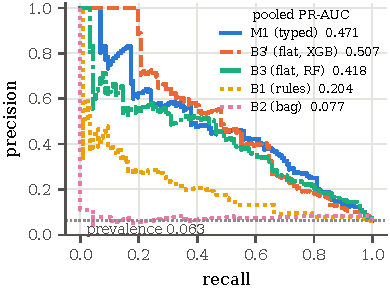
\includegraphics[width=\linewidth]{figures/fig3a.pdf}
\caption{Pooled PR curves.}
\label{fig:3a}
\end{subfigure}\hfill
\begin{subfigure}[t]{0.49\linewidth}\centering
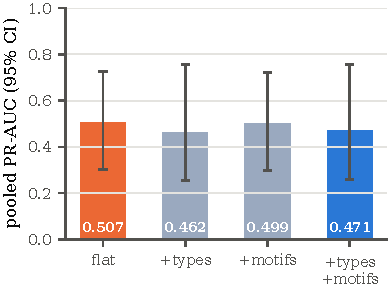
\includegraphics[width=\linewidth]{figures/fig3b.pdf}
\caption{Per-incident PR-AUC.}
\label{fig:3b}
\end{subfigure}\\[4pt]
\centering
\begin{subfigure}[t]{0.49\linewidth}\centering
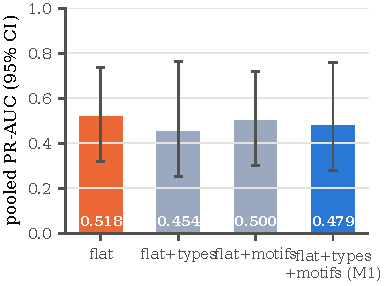
\includegraphics[width=\linewidth]{figures/fig3c.pdf}
\caption{Same learner, growing representation.}
\label{fig:3c}
\end{subfigure}
\caption{RQ1: detection over all prefixes. The learner is fixed in (c); only the feature groups change.}
\label{fig:rq1}
\end{figure}

\subsection{RQ2: How Early?}
\label{sec:rq2}

\paragraph{Online horizons.}
Figure~\ref{fig:4b} scores every trajectory at the prefix available $h$ minutes after its first action, which is what a live monitor sees.
One minute after the first action (median $k=2$ for incidents), M1 reaches PR-AUC 0.421 against 0.215 for B3$'$, a paired gain of $+0.206$ [0.032, 0.330], $p=0.010$.
The same holds at the absolute checkpoint $k=2$ (0.418 vs.\ 0.209, $+0.210$ [0.037, 0.333], $p=0.008$).
From five minutes on, the two representations are statistically indistinguishable, and from 30 minutes on (a median of nine incident actions) B3$'$ is numerically ahead, once amounts, fan-out and hop depth have had time to develop.
Both curves rise with the horizon, from about 0.4 in the first minute to 0.63--0.71 after one day.
Because we test eight horizons, the two significant early results would not survive a Bonferroni correction ($0.05/8=0.006$); we read them as consistent evidence, supported by both the online and the checkpoint view, that event types carry the signal when there is no structure yet.

\paragraph{Relative checkpoints.}
Figure~\ref{fig:4a} shows the retrospective view.
With a quarter of each trajectory observed M1 reaches 0.483 and with the complete trajectory 0.702 (B3$'$: 0.566 and 0.811); each checkpoint has 15 positive and 393 negative rows (3.7\% positive).
Figure~\ref{fig:4c} shows why early alerts are possible at all: the median calibrated score of incidents rises within the first 10\% of the trajectory and stays around 0.3--0.5, while the median negative stays near 0.03.

\begin{figure}[t]
\centering
\begin{subfigure}[t]{0.49\linewidth}\centering
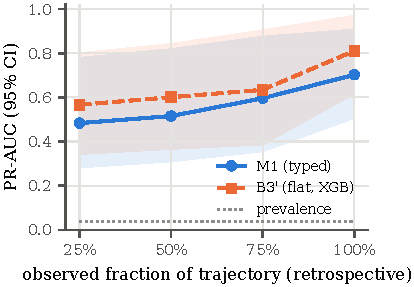
\includegraphics[width=\linewidth]{figures/fig4a.pdf}
\caption{Relative checkpoints.}
\label{fig:4a}
\end{subfigure}\hfill
\begin{subfigure}[t]{0.49\linewidth}\centering
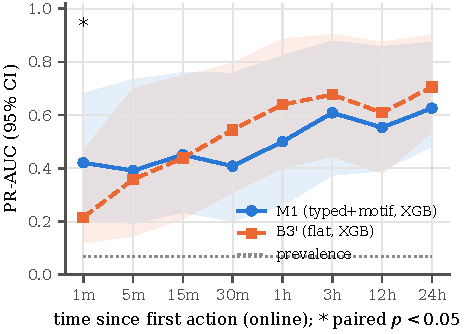
\includegraphics[width=\linewidth]{figures/fig4b.pdf}
\caption{Online horizons.}
\label{fig:4b}
\end{subfigure}\\[4pt]
\centering
\begin{subfigure}[t]{0.49\linewidth}\centering
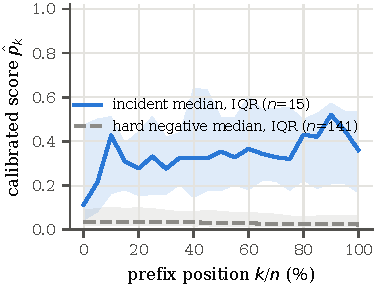
\includegraphics[width=\linewidth]{figures/fig4c.pdf}
\caption{Score along the trajectory.}
\label{fig:4c}
\end{subfigure}
\caption{RQ2: how early the signal appears. Shaded bands are incident-bootstrap 95\% CIs in (a,b) and interquartile ranges in (c).}
\label{fig:rq2}
\end{figure}

\paragraph{Alerts, lead time and false alerts.}
We replay every trajectory action by action, score each prefix $k\ge2$ with the calibrated M1 of its held-out fold, and record the first crossing of $\theta$ (Table~\ref{tab:lead}, Fig.~\ref{fig:rq2b}).
At $\theta=0.5$, 12 of 15 incidents raise an alert, and 12 of the 206 negatives that have at least two actions (5.8\%) raise a false alert; the other 187 negatives consist of a single action and are never scored.
Of the 10 incidents with a confirmed endpoint, three are alerted before the exit: DeltaPrime 114 minutes and six steps early, Chibi Finance 7.5 minutes and 17 steps early, and Radiant Capital 5 minutes and five steps early.
Four endpoints (FEG, New Free DAO, XKingdom, BSC Token Hub) are the \emph{first} action of the trace, the attacker sending the proceeds straight into a mixer, bridge or lending market, so no prefix-based detector can warn before them; of the six incidents where an early alert is possible, three receive one.
Raising $\theta$ trades detections for false alerts: at 0.7 the false-alert rate drops to 1.9\% but only one incident is alerted early.

\begin{table}[t]
\centering
\caption{RQ2: first alerts of calibrated M1 when every prefix $k\ge2$ is scored online. ``Before $t_e$'' counts the 10 incidents with a confirmed endpoint; 4 of them have their endpoint at $k=1$ and cannot be alerted early. False alerts are per trajectory over the 206 negatives with $\ge2$ actions.}
\label{tab:lead}
\small
\resizebox{\linewidth}{!}{%
\begin{tabular}{@{}lccccc@{}}
\toprule
$\theta$ & Before $t_e$ & Median lead [IQR] & Late / never & Incidents alerted & False-alert rate \\
\midrule
0.3 & 3/10 & 7.5 min [6.4, 60.5] & 6 / 1 & 14/15 & 12.6\% (26/206) \\
0.5 & 3/10 & 7.5 min [6.4, 60.5] & 5 / 2 & 12/15 & 5.8\% (12/206) \\
0.7 & 1/10 & 7.5 min & 2 / 7 & 5/15 & 1.9\% (4/206) \\
0.9 & 0/10 & -- & 0 / 10 & 0/15 & 0.0\% (0/206) \\
\bottomrule
\end{tabular}}
\end{table}

\begin{figure}[t]
\centering
\begin{subfigure}[t]{0.49\linewidth}\centering
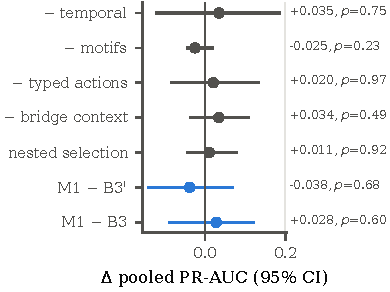
\includegraphics[width=\linewidth]{figures/fig5a.pdf}
\caption{Detection vs.\ false alerts.}
\label{fig:5a}
\end{subfigure}\hfill
\begin{subfigure}[t]{0.49\linewidth}\centering
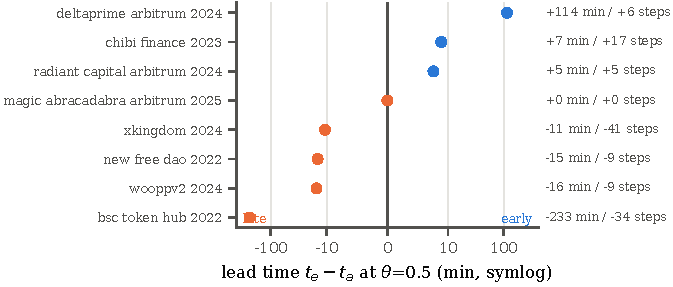
\includegraphics[width=\linewidth]{figures/fig5b.pdf}
\caption{Lead time per incident.}
\label{fig:5b}
\end{subfigure}\\[4pt]
\centering
\begin{subfigure}[t]{0.49\linewidth}\centering
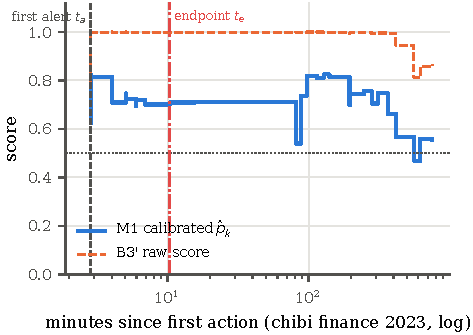
\includegraphics[width=\linewidth]{figures/fig5c.pdf}
\caption{Case study: Chibi Finance.}
\label{fig:5c}
\end{subfigure}
\caption{RQ2: alerting on the live replay. In (b) blue marks alerts before the endpoint and orange late alerts; incidents never alerted at $\theta=0.5$ are omitted.}
\label{fig:rq2b}
\end{figure}

\paragraph{Case study: Chibi Finance (2023).}
The exploiter of this Arbitrum rug pull made 40 actions in 12.6 hours; the endpoint is action 19, a Stargate bridge deposit 10 minutes after the first action (Fig.~\ref{fig:5c}).
After the second action, 2.8 minutes in, the calibrated score is 0.62 and the alert fires, 449\,s and 17 actions before the bridge deposit.
Its top TreeSHAP contributions are the mean log amount ($+1.50$), fan-out of the seed ($+0.84$) and a short mean gap between actions (170\,s, $+0.81$), followed by the absence of a bridge deposit so far ($+0.59$) and a swap share of 0.5 ($+0.53$): a large amount moving fast through a swap, i.e.\ AADAPT layering (ADT3028.003).
The score stays at or above 0.5 for 97\% of the remaining prefixes, through the bridge deposit and the following 12 hours.

\subsection{RQ3: Robustness, Calibration and Explanations}
\label{sec:rq3}

\paragraph{Ablations.}
Figure~\ref{fig:6a} removes one group at a time from M1.
No removal changes pooled PR-AUC significantly: temporal $+0.035$ ($p=0.75$), motifs $-0.025$ ($p=0.23$), typed actions $+0.020$ ($p=0.97$), bridge-context features $+0.034$ ($p=0.49$).
An earlier version of this pipeline dropped the bridge-context features after inspecting ablations on all incidents; choosing inside each training split instead (nested LOIO) keeps them in 3 of 15 folds and yields 0.490, within $0.011$ of M1 ($p=0.92$), so M1 as reported uses no post-hoc feature selection.

\paragraph{Calibration.}
Raw XGBoost scores are overconfident (ECE 0.071, Brier 0.075, Fig.~\ref{fig:6b}).
Platt scaling fitted on inner-fold scores reduces ECE to 0.015 [0.015, 0.071] and Brier to 0.062; isotonic regression reaches 0.021.
Calibrators are fitted per fold, so pooled PR-AUC over calibrated scores is lower (0.395) than over raw scores: calibration is used for thresholds and for the alert, not for ranking across folds.

\paragraph{Mimicry.}
We re-score each incident after inserting $j$ small decoy transfers to fresh addresses after every action (1\% of the value, one second apart), which dilutes type shares and motifs without changing the flow.
The fraction of incidents alerted within their first 400 actions falls from 80\% ($j=0$) to 60--67\% ($j\in\{1,2,4\}$), and the mean calibrated score at the 25\% checkpoint from 0.36 to 0.25 (Fig.~\ref{fig:6c}).
The detector degrades but is not blinded by cheap padding; an adaptive attacker who also slows down was not evaluated.

\paragraph{Builder settings.}
With one expansion round instead of two, trajectories are shorter (median 20 vs.\ 40 actions for incidents) and M1 is \emph{higher} (0.637--0.679 for $\eta\in\{5,10,20\}\%$) and above B3$'$ in all three settings (0.555--0.603).
With two rounds and $\eta\in\{10,20\}\%$, M1 is 0.554--0.566.
The ranking of M1 and B3$'$ thus depends on how far the trace is followed: deeper traces add long transfer chains in which amounts and hop depth dominate, while shallow traces keep the typed first steps in focus.

\begin{figure}[t]
\centering
\begin{subfigure}[t]{0.49\linewidth}\centering
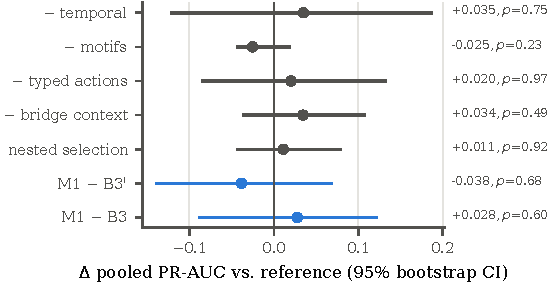
\includegraphics[width=\linewidth]{figures/fig6a.pdf}
\caption{Ablations (paired).}
\label{fig:6a}
\end{subfigure}\hfill
\begin{subfigure}[t]{0.49\linewidth}\centering
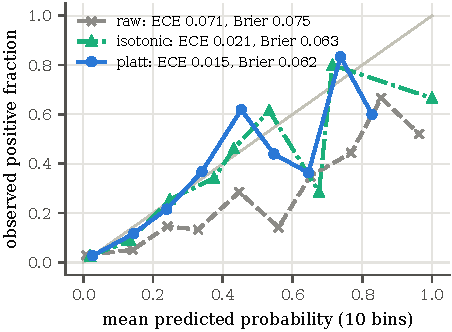
\includegraphics[width=\linewidth]{figures/fig6b.pdf}
\caption{Reliability diagram.}
\label{fig:6b}
\end{subfigure}\\[4pt]
\centering
\begin{subfigure}[t]{0.49\linewidth}\centering
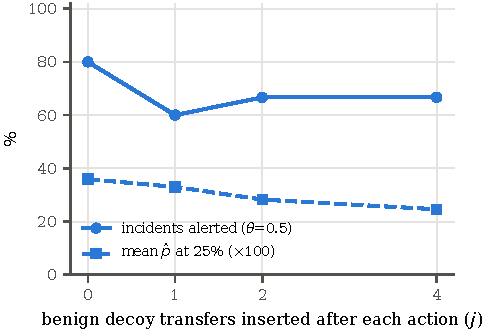
\includegraphics[width=\linewidth]{figures/fig6c.pdf}
\caption{Mimicry stress test.}
\label{fig:6c}
\end{subfigure}
\caption{RQ3: ablations, calibration and robustness to decoy transfers.}
\label{fig:rq3}
\end{figure}

\paragraph{What the model uses.}
Averaged over all prefixes (Fig.~\ref{fig:7a}), the largest TreeSHAP contributions come from the mean log amount, the bridge-deposit share, value retention, the mean gap between actions and the fan-out of the seed; typed features (bridge-deposit share, bigram diversity, transfer share, stablecoin legs) and the rapid-token-pivot motif make up five of the top twelve.
Stolen funds are large, move fast and leave the seed in few hops, whereas hard negatives are dominated by single bridge deposits of ordinary size (Fig.~\ref{fig:2b}).

\paragraph{Synthetic benchmark.}
On CAGI-Synth (Fig.~\ref{fig:7c}, synthetic data only), every learned detector reaches PR-AUC $\ge0.97$ at every difficulty, B1 stays below 0.18, and M1 trained on the real incidents and applied to synthetic data scores 0.014, below the synthetic prevalence (0.025).
Typology-based generators are thus \emph{easier} than real incidents and do not share their feature distribution; we release the generator as a sanity check and do not use synthetic results as evidence for any claim above.

\subsection{RQ4: Cost and Next-Action Forecasting}
\label{sec:rq4}

On a 4-core Intel Xeon at 2.1\,GHz, extracting the features of one prefix and scoring it takes a median of 11.7\,ms at $k=2$ and 23.6\,ms at $k=850$, with a peak memory increase below 0.2\,MB (Fig.~\ref{fig:7b}); re-scoring on every new action is far cheaper than the 12\,s Ethereum slot time, and end-to-end latency is dominated by the explorer API.
Before training a next-action model we fixed three data-sufficiency criteria: at least 1{,}000 transitions, at least 30 examples of each of the seven classes, and a majority class below 60\%.
The data pass the first (11{,}313 transitions) and fail the other two: transfers make up 67\% of transitions and lending deposits occur four times.
We therefore do not train a forecaster and report this as a negative result.

\begin{figure}[t]
\centering
\begin{subfigure}[t]{0.49\linewidth}\centering
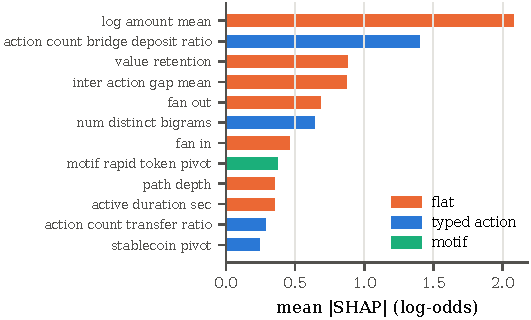
\includegraphics[width=\linewidth]{figures/fig7a.pdf}
\caption{Global TreeSHAP (top 12).}
\label{fig:7a}
\end{subfigure}\hfill
\begin{subfigure}[t]{0.49\linewidth}\centering
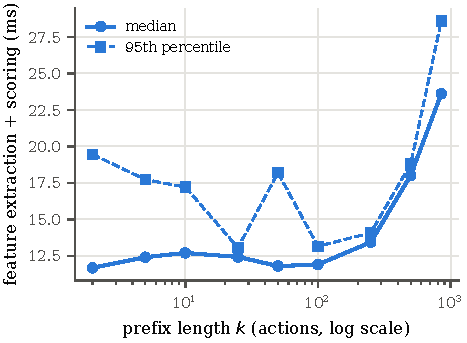
\includegraphics[width=\linewidth]{figures/fig7b.pdf}
\caption{Scoring latency on a CPU.}
\label{fig:7b}
\end{subfigure}\\[4pt]
\centering
\begin{subfigure}[t]{0.49\linewidth}\centering
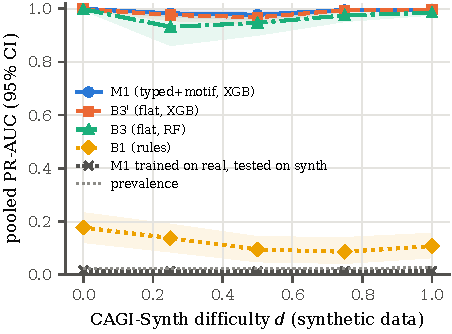
\includegraphics[width=\linewidth]{figures/fig7c.pdf}
\caption{CAGI-Synth (synthetic only).}
\label{fig:7c}
\end{subfigure}
\caption{What the model uses, what it costs, and the synthetic sanity benchmark.}
\label{fig:rq4}
\end{figure}
%=============================================================================
\section{Discussion}
\label{sec:discussion}
%=============================================================================

\paragraph{What the evidence supports.}
Early warning on real cross-chain incidents is feasible but hard.
A calibrated detector alerts on 12 of 15 incidents at a 5.8\% per-trajectory false-alert rate on hard negatives drawn from the same bridges and DEXs, and in three of the six incidents where an early alert is possible at all it fires 5 to 114 minutes before the exit.
The typed representation earns its keep in the first minute of a flow, where it doubles PR-AUC over the same learner on flat features; once a flow has a few dozen actions, amounts, tempo and hop structure carry the signal and typing adds nothing measurable at $N=15$.
Rule-based typology scores, the natural first tool of a compliance team, are far weaker than any learned detector.
We therefore see the main value of typing in the \emph{earliest} alert and in its explanation: an analyst receives ``large amount, swap then fan-out within three minutes (ADT3028.003 Layering)'' rather than an opaque score.

\paragraph{What changed from our earlier analysis.}
Re-building the pipeline for this paper exposed three problems in our own earlier version, and we report them because they are easy to repeat.
(i) A relative-position feature $k/n$ leaked the final trajectory length into every prefix.
(ii) Incidents were expanded six hops and negatives two, so hop depth and length separated the classes by construction.
(iii) A feature group was dropped after inspecting ablations on all incidents.
Together with the re-collected data, correcting them lowered the typed model's pooled PR-AUC from 0.736 in our earlier draft to the 0.479 reported here.
The unit test that compares prefixes of trajectories with different futures, uniform expansion for all trajectories, and nested selection now guard against these errors.

\paragraph{Limitations and threats to validity.}
\emph{Sample size.} Fifteen incidents give wide intervals; most group-level differences are not significant, and the two significant early-horizon results do not survive a Bonferroni correction over eight horizons.
\emph{Incomplete BSC negatives.} The free NodeReal quota ran out, so BSC incidents have fewer negatives (0 to 23) than Ethereum and Arbitrum incidents (24 to 75), two incidents have none, and one incident is rebuilt from an earlier trace.
\emph{Selection bias.} Incidents come from public reports, which over-represent large, well-investigated thefts; the strong role of amount features partly reflects this.
\emph{Scope.} Traces follow one chain to two expansion rounds; bridge exits are endpoints rather than stitched continuations, and non-EVM chains need new decoders.
\emph{Endpoint definition.} We use the first exit action in the trace; for four incidents this is the first action, and for two incidents the reported exit lies outside the traced depth.
\emph{Adaptive adversaries.} Cheap decoy transfers reduce detection from 80\% to 60--67\%; an attacker who also imitates benign tempo and amounts was not evaluated, and our synthetic generator shows that hand-written typologies do not reproduce the difficulty of real data.
\emph{Offline replay.} Detection is evaluated by replaying cached data in time order, not on a live stream.

\paragraph{Ethics.}
CAGI-ED uses public on-chain data and labels from public reports only.
It performs no de-anonymization beyond those sources and uses no exchange or proprietary labels.
Alerts are calibrated, explained signals for human review under AML obligations for virtual-asset service providers~\cite{fatf2022targeted}, not automatic enforcement, because a false alert affects a legitimate user.

\paragraph{Availability.}
The incident and negative registries, the raw API responses with checksums, the decoded trajectories, all per-incident results and the scripts that regenerate every number and figure from one command are available at \TBD{anonymous artifact URL}.

%=============================================================================
\section{Conclusion}
\label{sec:conclusion}
%=============================================================================

We framed cross-chain laundering analysis as early detection on trajectory prefixes and built CAGI-ED, a CPU-only pipeline from explorer APIs to calibrated, explained alerts.
On 15 real incidents with 393 hard negatives from the same protocols, it alerts on most incidents at a low false-alert rate and, where the flow leaves time, minutes to hours before the exit.
Typing each action by its DeFi semantics helps most at the very first steps of a flow and in explaining alerts, while amount, tempo and hop structure dominate later; a rule-based typology score is not a substitute for either.
A larger set of incidents with complete negatives is the most important next step, followed by stitching bridge continuations across chains, evaluating against adaptive adversaries on a live stream, and revisiting next-action forecasting once enough labeled exits exist.

\bibliographystyle{splncs04}
\bibliography{refs}

\appendix
\section{Incident Registry}
\label{app:incidents}
Table~\ref{tab:incidents} lists the incidents in chronological order. Full addresses, block numbers, transaction hashes of the evidence and all source links are in the file \path{metadata/incident_registry.csv} of the artifact.
% BEGIN auto:incident-table (regenerated by scripts/make_figures.py)
\begin{table}[h]
\centering
\caption{The 15 incidents. $n$: actions in the trajectory; endpoint: type and index $e^\star$ of the first exit action in the trace (-- if the confirmed exit lies outside the traced chain or depth); Neg.: hard negatives with a complete cache. $^\dagger$ rebuilt from our earlier decoded trace (Sect.~\ref{sec:data}).}
\label{tab:incidents}
\scriptsize
\setlength{\tabcolsep}{2.5pt}
\resizebox{\linewidth}{!}{%
\begin{tabular}{@{}lllcrrlrp{3.0cm}@{}}
\toprule
Incident & Start & Chain & Seed & $n$ & Hours & Endpoint ($e^\star$) & Neg. & Public sources \\
\midrule
Wault Finance & 2021-08-04 & BSC & 0x886358\ldots & 37 & 68.6 & -- (--) & 6 & SlowMist \\
Qubit QBridge & 2022-01-27 & BSC & 0xd01ae1\ldots & 643 & 71.6 & -- (--) & 13 & CertiK;  SlowMist \\
Paraluni$^\dagger$ & 2022-03-12 & BSC & 0x94bc1d\ldots & 425 & 71.9 & -- (--) & 1 & CertiK;  SlowMist \\
Ronin Bridge & 2022-03-23 & ETH & 0x098b71\ldots & 331 & 48.2 & -- (--) & 75 & Ronin Network official disclosure;  Chainalysis \\
HackerDAO & 2022-04-29 & BSC & 0xcfc591\ldots & 35 & 60.8 & -- (--) & 0 & CertiK Hackerdao Incident Analysis \\
New Free DAO & 2022-05-10 & BSC & 0x22c973\ldots & 12 & 0.3 & mixer or exit (1) & 0 & Halborn;  ImmuneBytes \\
BSC Token Hub & 2022-10-06 & BSC & 0x489a87\ldots & 364 & 63.7 & lending deposit (1) & 23 & Halborn;  Merkle Science \\
Chibi Finance & 2023-06-27 & ARB & 0x80c1ca\ldots & 40 & 12.6 & bridge deposit (19) & 34 & CertiK \\
XKingdom & 2024-01-06 & ARB & 0xef7dd2\ldots & 68 & 4.8 & bridge deposit (1) & 32 & CertiK \\
WOOFi WooPPV2 & 2024-03-05 & ARB & 0x996119\ldots & 16 & 0.7 & bridge deposit (5) & 35 & Beosin;  CUBE3.AI \\
UtopiaSphere & 2024-07-21 & BSC & 0x6e12ce\ldots & 37 & 42.5 & bridge deposit (10) & 8 & CertiK \\
Radiant Capital & 2024-10-16 & ARB & 0x0629b1\ldots & 243 & 22.2 & bridge deposit (7) & 25 & Halborn official post-mortem analysis;  CoinDesk \\
DeltaPrime & 2024-11-11 & ARB & 0x56e7f6\ldots & 22 & 23.3 & bridge deposit (8) & 75 & CertiK official incident analysis;  Halborn \\
FEG SmartBridge & 2024-12-29 & ETH & 0xcb96dd\ldots & 9 & 0.2 & mixer or exit (1) & 42 & CertiK;  Halborn \\
Abracadabra (MIM) & 2025-03-25 & ARB & 0x51c9d0\ldots & 90 & 12.7 & bridge deposit (31) & 24 & CertiK;  threesigma.xyz Abracadabra GMX V2 exploit analysis \\
\bottomrule
\end{tabular}}
\end{table}
% END auto:incident-table

\end{document}
